\newpage
\subsection{Altitude Variations}
This series of tests involved evaluating the effect of uniformly changing the altitudes of each satellite from the reference case specified in Table \ref{tab:satRefCase} on the performance metrics outlined in Section \ref{sec:perfMetrics}.
\subsubsection{Input Variables}
From the reference case specified in Table \ref{tab:satRefCase}, the altitudes of each satellite were varied between 400km and 800km in 50km steps according to Table \ref{tab:altitudeParams}.

\begin{table}[H]
  \centering
  \caption{Altitude variations used}
    \begin{tabular}{p{2.5cm}rr}
    \toprule
    Case Number & Altitude (km) & Semi-Major Axis (km)\\
    \midrule
    1     & 400   & 6778.14 \\
    2     & 450   & 6828.14 \\
    3     & 500   & 6878.14 \\
    4     & 550   & 6928.14 \\
    5     & 600   & 6978.14 \\
    6     & 650   & 7028.14 \\
    7     & 700   & 7078.14 \\
    8     & 750   & 7128.14 \\
    9     & 800   & 7178.14 \\

    \bottomrule
    \end{tabular}%
  \label{tab:altitudeParams}%
\end{table}%
All other orbital parameters remained constant as per Table \ref{tab:satRefCase}.

After initial testing, it was hypothesised that the high number of satellites in the reference constellation was causing a high degree of overlap between coverage from different satellites. This phenomenon would pollute the observed trend of the access-coverage behaviour. The set of experiments was therefore repeated using a smaller 3 satellite constellation with orbital parameters specified in Table \ref{tab:3sat_config}. The range of altitudes tested was the same as specified in Table \ref{tab:altitudeParams}.
% Table generated by Excel2LaTeX from sheet 'Sheet1'
\begin{table}[htbp]
  \centering
  \caption{Orbital parameters for 3 satellite test}
    \begin{tabular}{rrr}
    \toprule
    Satellite & RAAN  & True Anomaly \\
    \midrule
    1     & 0     & 0 \\
    2     & 120   & 120 \\
    3     & 240   & 240 \\
    \bottomrule
    \end{tabular}%
  \label{tab:3sat_config}%
\end{table}%



\subsubsection{Trends}
The results for altitude variations against the resulting coverage gap fractions, maximum gap period and minimum received signal power are shown in Figures \ref{fig:AltitudeVsCovGap12sat}, \ref{fig:AltitudeVsMaxGap12sat} and \ref{fig:AltitudeVsRxPower12sat} respectively. The results show that the coverage gap fraction and maximum coverage gap become lower with a higher satellite altitude. Similarly the minimum received isotropic power was reduced with higher altitude.  The coverage trends for the repeated three-satellite constellation test are given in Figures \ref{fig:AltitudeVsCovGap3sat} and \ref{fig:AltitudeVsMaxGap3sat}, showing the same trends.
\begin{figure}[htbp]
	\centering
	\includegraphics[scale = 0.6]{Pictures/AltitudeVsCovGap12sat.png}
	
	\caption{Coverage gap (as a fraction of total analysis time) as effected by altitude variations. Lower is better}
	\label{fig:AltitudeVsCovGap12sat}
\end{figure} 


\begin{figure}[htbp]
	\centering
	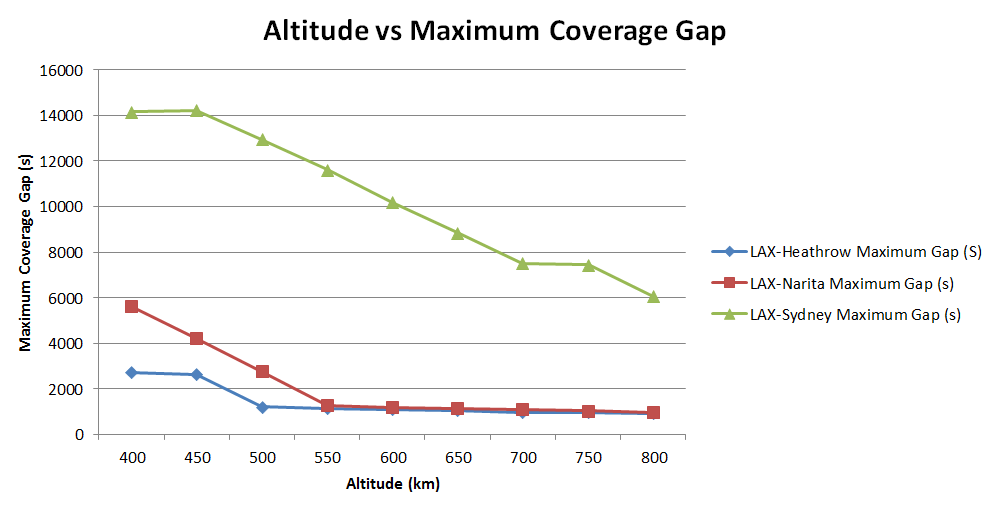
\includegraphics[scale = 0.6]{Pictures/AltitudeVsMaxGap12sat.png}
	
	\caption{Maximum coverage gap as affected by altitude variations. Lower is better}
	\label{fig:AltitudeVsMaxGap12sat}
\end{figure} 

\begin{figure}[htbp]
	\centering
	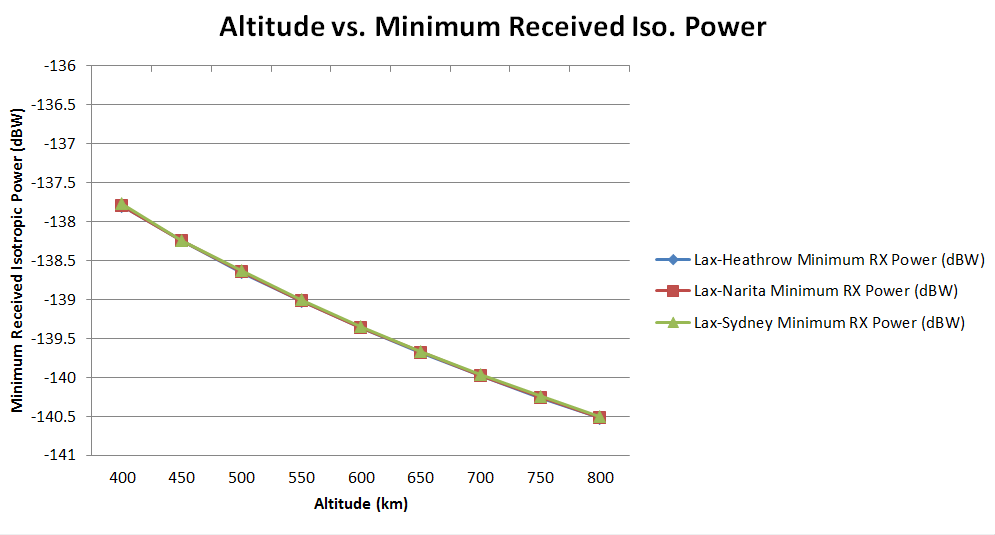
\includegraphics[scale = 0.6]{Pictures/AltitudeVsRxPower12sat.png}
	
	\caption{Minimum received isotropic power as affected by altitude variations. Higher is better.}
	\label{fig:AltitudeVsRxPower12sat}
\end{figure}


\begin{figure}[htbp]
	\centering
	\includegraphics[scale = 0.6]{Pictures/AltitudeVsCovGap3sat.png}
	
	\caption{Coverage gap (as a fraction of total analysis time) as effected by altitude variations with a 3 satellite constellation. Lower is better}
	\label{fig:AltitudeVsCovGap3sat}
\end{figure} 


\begin{figure}[htbp]
	\centering
	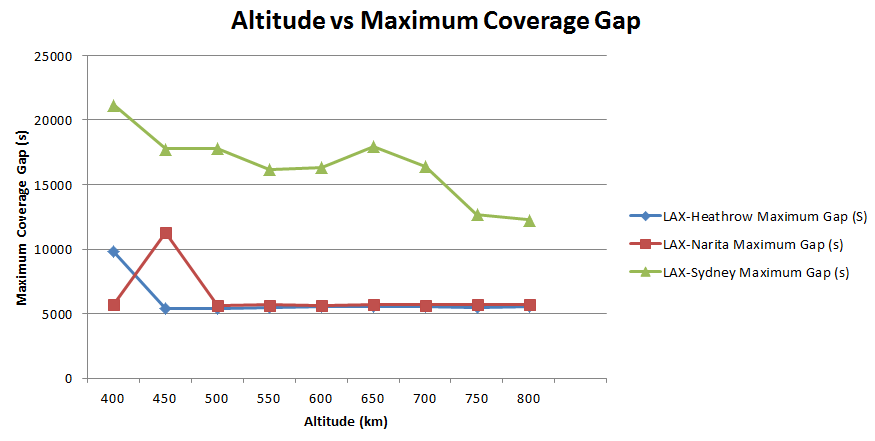
\includegraphics[scale = 0.6]{Pictures/AltitudeVsMaxGap3sat.png}
	
	\caption{Maximum coverage gap as affected by altitude variations retested with a 3 satellite constellation. Lower is better. }
	\label{fig:AltitudeVsMaxGap3sat}
\end{figure} 

\subsubsection{Discussion}
The results for both coverage gap times and received RF power behaved as expected. Satellites at higher altitudes have a greater line of sight range \footnote{The area on Earth within which objects will have a direct line of sight toward a satellite, allowing for a simple RF link to be made.} increasing the probability with which any one flight could be `seen' by a satellite. The difference in orbital period between the extremes of altitude (1 hour and 32.5 minutes at 800km against 1 hour and 42.9 minutes at 400 km) was less than 10\% and had minimal effect on the periodicity of access times. The net effect was the observed increase in coverage time and decrease of coverage gaps for any given flight path. The trends observed in the coverage-access times for the three-satellite test shown in Figures \ref{fig:AltitudeVsCovGap3sat} and \ref{fig:AltitudeVsMaxGap3sat} matched those quite closely with those seen in the reference case with 12 satellites. This indicated that the number of satellites did not affect the trend observed in either case

There was a significant observed difference in coverage gaps for the flights between LAX and Sydney and LAX and Heathrow or Narita. The maximum coverage gaps for LAX-Sydney were worse by one order of magnitude of time, as is shown in Figure \ref{fig:AltitudeVsMaxGap12sat}. This is due to the fact that 60 degree inclination of the satellites resulted in ground tracks that were almost coincident with the flight paths between LAX and Narita or Heathrow, as can be seen in Figure \ref{fig:12sat_60deg_flightPaths}. The geometry of the ground tracks was not optimised for the flight path between LAX and Sydney, resulting in a less desirable maximum coverage gap.

\begin{figure}[htbp]
	\centering
	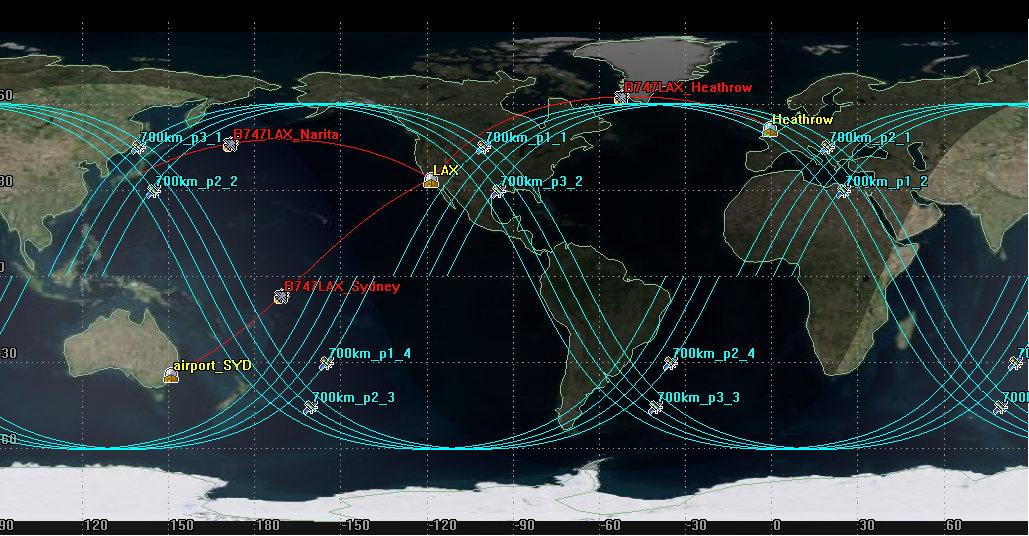
\includegraphics[scale = 0.6]{Pictures/12sat_60deg_flightPaths.png}
	
	\caption{Ground track of satellites inclined at 60 degrees, shown with the test flight paths}
	\label{fig:12sat_60deg_flightPaths}
\end{figure} 

Despite the increased access time at higher altitudes, however, a significant drop in received signal strength is observed between 400km and 800km altitude. There was an expected drop due to the increased distance and subsequent increased free-space path loss of any electromagnetic wave.  The minimum received isotropic power is optimised at 400km, with a measurement of -137.8 dBW and is the least optimised at 800km with a measurement of -140.5 dBW. This is a difference of 2.7 dBW, meaning that from 400km altitude to 800km altitude, the raw signal power has been reduced by a factor of 1.86. This will affect ADS-B detectability as weaker signals will be harder to detect and process. The effect of this on the performance of the system is evaluated later in Section \ref{sec:decision_matrix}.

The minimum trigger threshold level for an ADS-B receiver class R3 (Extended) as specified by the RTCA is set at -84 dBm \cite{RTCA_MODE_S} or equivalently -114 dBW. This is already well above that reported possible with the standard STK transmitter-receiver model at 400 km altitude. 


  
 